\documentclass[12pt,letterpaper]{report}
\usepackage[spanish]{babel}
\usepackage[utf8]{inputenc}
\usepackage{graphicx}
\usepackage{hyperref}
\usepackage{listings}
\usepackage{xcolor}
\usepackage{geometry}
\usepackage{titlesec}
\usepackage{fancyhdr}
\usepackage{tocloft}
\usepackage{bookmark}

% Configuración de geometría de página
\geometry{margin=2.5cm}

% Configuración de colores
\definecolor{codegreen}{rgb}{0,0.6,0}
\definecolor{codegray}{rgb}{0.5,0.5,0.5}
\definecolor{codepurple}{rgb}{0.58,0,0.82}
\definecolor{backcolour}{rgb}{0.95,0.95,0.92}

% Configuración de listings para código
\lstdefinestyle{mystyle}{
    backgroundcolor=\color{backcolour},   
    commentstyle=\color{codegreen},
    keywordstyle=\color{magenta},
    numberstyle=\tiny\color{codegray},
    stringstyle=\color{codepurple},
    basicstyle=\ttfamily\footnotesize,
    breakatwhitespace=false,         
    breaklines=true,                 
    captionpos=b,                    
    keepspaces=true,                 
    numbers=left,                    
    numbersep=5pt,                  
    showspaces=false,                
    showstringspaces=false,
    showtabs=false,                  
    tabsize=2
}

\lstset{style=mystyle}

% Configuración de encabezados y pies de página
\pagestyle{fancy}
\fancyhf{}
\fancyhead[L]{API de Dispositivos IoT}
\fancyhead[R]{\thepage}
\fancyfoot[C]{Universidad Autónoma de Tamaulipas}

% Configuración de la tabla de contenidos
\renewcommand{\cftchapfont}{\bfseries}
\renewcommand{\cftchappagefont}{\bfseries}
\renewcommand{\cftchapdotsep}{\cftdotsep}
\setlength{\cftbeforechapskip}{1em}
\setlength{\cftbeforesecskip}{0.5em}
\setlength{\cftbeforesubsecskip}{0.25em}
\renewcommand{\cftchapafterpnum}{\vskip5pt}
\renewcommand{\cftsecafterpnum}{\vskip3pt}

% Configuración de bookmarks para PDF
\bookmarksetup{
  numbered,
  open,
  depth=3
}

\begin{document}

% Portada
\begin{titlepage}
    \centering
    \vspace*{1cm}
    {\Huge\bfseries Documentación de API FastAPI\\para Dispositivos IoT\par}
    \vspace{2cm}
    {\Large\itshape Diseño de Sistemas Embebidos\par}
    \vspace{3cm}

    % Aquí debes insertar el logo de tu escuela
    % Reemplaza "logo_escuela.png" con la ruta a tu logo
    % Comentado para permitir la compilación sin el archivo de logo
    
\includegraphics[width=0.5\textwidth]{logo_uat}\\

    \vspace{3cm}

    {\Large\bfseries Universidad Autónoma de Tamaulipas\par}
    \vspace{0.5cm}
    {\large Facultad de Ingeniería\par}
    \vspace{1.5cm}

    % Aquí debes incluir los nombres de los miembros del equipo
    {\large\bfseries Equipo:\par}
    \vspace{0.5cm}
    {\large Juan Julián Paniagua Rico - a2213332303\par}
    {\large Isaac Sayeg Posadas Perez - a2213332197\par}
    {\large Jorge Roberto Garcia Azzua - a2221335006\par}
    \vspace{1.5cm}

    {\large \today\par}
\end{titlepage}

% Tabla de contenidos
\cleardoublepage
\phantomsection
\addcontentsline{toc}{chapter}{Índice de Contenidos}
\renewcommand{\contentsname}{Índice de Contenidos}
\setcounter{tocdepth}{3}
\setcounter{secnumdepth}{3}

\begin{center}
    \vspace*{1cm}
    {\Huge\bfseries Índice de Contenidos}
    \vspace{0.5cm}

    \noindent\makebox[\linewidth]{\rule{\textwidth}{0.4pt}}
    \vspace{1cm}
\end{center}

\tableofcontents
\thispagestyle{fancy}

\newpage

\chapter{Introducción}

\section{Descripción General}
Esta documentación describe una aplicación FastAPI para gestionar dispositivos IoT y sus registros. La API proporciona operaciones CRUD (Crear, Leer, Actualizar, Eliminar) para varios tipos de dispositivos y sus datos.

FastAPI es un framework moderno y de alto rendimiento para construir APIs con Python 3.7+. Se basa en estándares abiertos como OpenAPI y JSON Schema, y proporciona características como validación automática, serialización, documentación interactiva y mucho más.

\section{Características Principales}
La API de Dispositivos IoT ofrece las siguientes características principales:

\begin{itemize}
    \item Gestión completa de dispositivos IoT con operaciones CRUD
    \item Registro y seguimiento de datos de dispositivos
    \item Soporte para diferentes tipos de dispositivos (luces, controladores de voltaje, etc.)
    \item Documentación interactiva con Swagger UI y ReDoc
    \item Validación automática de datos con Pydantic
    \item Persistencia de datos con SQLAlchemy
\end{itemize}

Esta documentación incluye ejemplos de código, explicaciones detalladas de los endpoints y modelos de datos, así como evidencias visuales de la ejecución del código en el Capítulo 7, que muestran el funcionamiento real de la API.

\chapter{Instalación y Configuración}

\section{Requisitos Previos}
Para ejecutar la API, necesitarás:

\begin{itemize}
    \item Python 3.7 o superior
    \item pip (gestor de paquetes de Python)
    \item Acceso a una base de datos (SQLite por defecto)
\end{itemize}

\section{Instalación de Dependencias}
Instala las dependencias requeridas con el siguiente comando:

\begin{lstlisting}[language=bash]
pip install fastapi uvicorn sqlalchemy pydantic python-dotenv
\end{lstlisting}

\section{Configuración de la Base de Datos}
La aplicación utiliza SQLAlchemy como ORM (Object-Relational Mapping) para interactuar con la base de datos. Por defecto, se configura para usar SQLite, pero puede configurarse para usar otras bases de datos.

Configura tu conexión a la base de datos en el archivo \texttt{.env}:

\begin{lstlisting}
DATABASE_URL=sqlite:///./iot_devices.db
\end{lstlisting}

Para usar otras bases de datos, modifica la URL según el formato requerido por SQLAlchemy.

\section{Ejecución de la API}
Para ejecutar la API, utiliza el siguiente comando desde el directorio \texttt{server}:

\begin{lstlisting}[language=bash]
uvicorn main:app --reload
\end{lstlisting}

Esto iniciará el servidor en \texttt{http://localhost:8000}. La opción \texttt{--reload} permite que el servidor se reinicie automáticamente cuando detecta cambios en el código.

\chapter{Arquitectura de la Aplicación}

\section{Estructura del Proyecto}
La aplicación sigue una estructura modular con los siguientes componentes principales:

\begin{itemize}
    \item \texttt{main.py}: Punto de entrada de la aplicación y definición de endpoints
    \item \texttt{models.py}: Definición de modelos de datos (SQLAlchemy y Pydantic)
    \item \texttt{database.py}: Configuración de la conexión a la base de datos
    \item \texttt{crud.py}: Operaciones CRUD para interactuar con la base de datos
\end{itemize}

\section{Flujo de Datos}
El flujo de datos en la aplicación sigue este patrón:

\begin{enumerate}
    \item El cliente envía una solicitud HTTP a un endpoint específico
    \item FastAPI valida la solicitud utilizando los modelos Pydantic
    \item El controlador (función en \texttt{main.py}) procesa la solicitud
    \item Se realizan operaciones CRUD en la base de datos según sea necesario
    \item Se devuelve una respuesta al cliente, validada por los modelos Pydantic
\end{enumerate}

\chapter{Modelos de Datos}

\section{Modelos SQLAlchemy}
Los modelos SQLAlchemy definen la estructura de las tablas en la base de datos:

\subsection{DevicesInfoDB}
Almacena información básica sobre los dispositivos:

\begin{lstlisting}[language=python]
    from sqlalchemy import Base,Column,Integer,Numeric,String
class DevicesInfoDB(Base):
    __tablename__ = "DevicesInfo"
    id_device = Column(Integer, primary_key=True, index=True, nullable=False, unique=True, autoincrement=True)
    id_type = Column(Numeric, primary_key=False, index=False, nullable=False, unique=True, autoincrement=False)
    id_signal_type = Column(Numeric, primary_key=False, index=False, nullable=False, unique=True, autoincrement=False)
    nombre = Column(String, unique=False, index=True, nullable=False)
    vendor = Column(String, unique=False, index=True, nullable=False)
\end{lstlisting}

\subsection{DevicesRecordsDB}
Almacena registros de datos de los dispositivos:

\begin{lstlisting}[language=python]
    from sqlalchemy import Base,Column,Integer,Numeric,String,Date
class DevicesRecordsDB(Base):
    __tablename__ = "DevicesRecords"
    id_record = Column(Integer, primary_key=True, index=True, nullable=False, unique=True, autoincrement=True)
    id_device = Column(Numeric, primary_key=False, index=False, nullable=False, unique=False, autoincrement=False)
    current_value = Column(Numeric, index=False, unique=False, nullable=False)
    date_record = Column(Date, index=False, unique=False, nullable=False)
\end{lstlisting}

\subsection{TomaDecisionesDB}
Almacena decisiones basadas en datos:

\begin{lstlisting}[language=python]
    from sqlalchemy import Base,Column,Integer,Numeric,String,Date
class TomaDecisionesDB(Base):
    __tablename__ = "TomaDecisiones"
    id_decision = Column(Integer, primary_key=True, index=True, nullable=False, unique=True, autoincrement=True)
    velocidad = Column(Numeric, index=False, unique=False, nullable=False)
    decision = Column(Numeric, index=False, unique=False, nullable=False)
    date_record = Column(Date, index=False, unique=False, nullable=False)
\end{lstlisting}

\subsection{LucesDB}
Almacena información específica de dispositivos de iluminación:

\begin{lstlisting}[language=python]
    from sqlalchemy import Base,Column,Integer,Numeric,String
class LucesDB(Base):
    __tablename__ = "Luces"
    id_device = Column(Integer, primary_key=True, index=True, nullable=False, unique=True, autoincrement=True)
    lumens = Column(Numeric, index=False, unique=False, nullable=False)
    nombre = Column(String, unique=False, index=True, nullable=False)
    vendor = Column(String, unique=False, index=True, nullable=False)
\end{lstlisting}

\subsection{ControladorVoltajeDB}
Almacena información específica de controladores de voltaje:

\begin{lstlisting}[language=python]
    from sqlalchemy import Base,Column,Integer,Numeric,String
class ControladorVoltajeDB(Base):
    __tablename__ = "ControladorVoltaje"
    id_device = Column(Integer, primary_key=True, index=True, nullable=False, unique=True, autoincrement=True)
    encendido = Column(Integer, index=False, unique=False, nullable=False)  # Usa Integer para booleano
    voltaje = Column(Numeric, index=False, unique=False, nullable=False)
    nombre = Column(String, unique=False, index=True, nullable=False)
    vendor = Column(String, unique=False, index=True, nullable=False)
\end{lstlisting}

\section{Modelos Pydantic}
Los modelos Pydantic se utilizan para validar datos de entrada y salida en la API:

\subsection{DevicesInfo y DevicesInfoResponse}
\begin{lstlisting}[language=python]
    from pydantic import BaseModel
class DevicesInfo(BaseModel):
    id_device: int
    id_type: int
    id_signal_type: int
    nombre: str
    vendor: str

class DevicesInfoResponse(BaseModel):
    id_device: int
    id_type: float
    id_signal_type: float
    nombre: str
    vendor: str

    class Config:
        from_attributes = True
\end{lstlisting}

\subsection{DevicesRecords y DevicesRecordsResponse}
\begin{lstlisting}[language=python]
    from pydantic import BaseModel,datetime
class DevicesRecords(BaseModel):
    id_record: int
    id_device: int
    current_value: float
    date_record: datetime

class DevicesRecordsResponse(BaseModel):
    id_record: int
    id_device: float
    current_value: float
    date_record: datetime

    class Config:
        from_attributes = True
\end{lstlisting}

\subsection{TomaDecisiones y TomaDecisionesResponse}
\begin{lstlisting}[language=python]
    from pydantic import  BaseModel
from datetime import datetime
class TomaDecisiones(BaseModel):
    id_decision: int
    velocidad: float
    decision: float
    date_record: datetime

class TomaDecisionesResponse(BaseModel):
    id_decision: int
    velocidad: float
    decision: float
    date_record: datetime

    class Config:
        from_attributes = True
\end{lstlisting}

\subsection{Luces y LucesResponse}
\begin{lstlisting}[language=python]
    from pydantic import BaseModel
class Luces(BaseModel):
    lumens: float
    id_device: int
    nombre: str
    vendor: str

class LucesResponse(BaseModel):
    id_device: int
    lumens: float
    nombre: str
    vendor: str

    class Config:
        from_attributes = True
\end{lstlisting}

\subsection{ControladorVoltaje y ControladorVoltajeResponse}
\begin{lstlisting}[language=python]
    from pydantic import  BaseModel
class ControladorVoltaje(BaseModel):
    encendido: bool
    voltaje: float
    id_device: int
    nombre: str
    vendor: str

class ControladorVoltajeResponse(BaseModel):
    id_device: int
    encendido: bool
    voltaje: float
    nombre: str
    vendor: str

    class Config:
        from_attributes = True
\end{lstlisting}

\chapter{Endpoints de la API}

\section{Endpoint Raíz}
\begin{itemize}
    \item \textbf{GET /}
    \item \textbf{Descripción:} Devuelve un mensaje de bienvenida
    \item \textbf{Respuesta:} \texttt{\{"message": "Bienvenido a la API de Dispositivos IoT"\}}
\end{itemize}

\section{Endpoints de Test}
\subsection{GET /tests/}
\begin{itemize}
    \item \textbf{Descripción:} Obtiene todos los tests
    \item \textbf{Respuesta:} Lista de objetos TestModel
\end{itemize}

\subsection{GET /tests/\{test\_id\}}
\begin{itemize}
    \item \textbf{Descripción:} Obtiene un test por ID
    \item \textbf{Parámetros:} test\_id (entero)
    \item \textbf{Respuesta:} Objeto TestModel
\end{itemize}

\subsection{POST /tests/?title=\{title\}}
\begin{itemize}
    \item \textbf{Descripción:} Crea un nuevo test
    \item \textbf{Parámetros:} title (cadena)
    \item \textbf{Respuesta:} Objeto TestModel creado
\end{itemize}

\subsection{DELETE /tests/\{test\_id\}}
\begin{itemize}
    \item \textbf{Descripción:} Elimina un test
    \item \textbf{Parámetros:} test\_id (entero)
    \item \textbf{Respuesta:} Mensaje de confirmación
\end{itemize}

\section{Endpoints de DevicesInfo}
\subsection{GET /devices/info/}
\begin{itemize}
    \item \textbf{Descripción:} Obtiene información de todos los dispositivos
    \item \textbf{Respuesta:} Lista de objetos DevicesInfoResponse
\end{itemize}

\subsection{GET /devices/info/\{id\_device\}}
\begin{itemize}
    \item \textbf{Descripción:} Obtiene información de un dispositivo por ID
    \item \textbf{Parámetros:} id\_device (entero)
    \item \textbf{Respuesta:} Lista de objetos DevicesInfoResponse
\end{itemize}

\subsection{POST /devices/info/}
\begin{itemize}
    \item \textbf{Descripción:} Crea información de un nuevo dispositivo
    \item \textbf{Cuerpo:} Objeto DevicesInfo
    \item \textbf{Respuesta:} Objeto DevicesInfoResponse creado
\end{itemize}

\subsection{PUT /devices/info/\{id\_device\}}
\begin{itemize}
    \item \textbf{Descripción:} Actualiza información de un dispositivo
    \item \textbf{Parámetros:} id\_device (entero)
    \item \textbf{Cuerpo:} Objeto DevicesInfo
    \item \textbf{Respuesta:} Objeto DevicesInfoResponse actualizado
\end{itemize}

\subsection{DELETE /devices/info/\{id\_device\}}
\begin{itemize}
    \item \textbf{Descripción:} Elimina información de un dispositivo
    \item \textbf{Parámetros:} id\_device (entero)
    \item \textbf{Respuesta:} Mensaje de confirmación
\end{itemize}

\section{Endpoints de DevicesRecords}
\subsection{GET /devices/records/}
\begin{itemize}
    \item \textbf{Descripción:} Obtiene todos los registros de dispositivos
    \item \textbf{Respuesta:} Lista de objetos DevicesRecordsResponse
\end{itemize}

\subsection{GET /devices/records/\{id\_record\}}
\begin{itemize}
    \item \textbf{Descripción:} Obtiene un registro de dispositivo por ID
    \item \textbf{Parámetros:} id\_record (entero)
    \item \textbf{Respuesta:} Objeto DevicesRecordsResponse
\end{itemize}

\subsection{GET /devices/records/device/\{id\_device\}}
\begin{itemize}
    \item \textbf{Descripción:} Obtiene registros de dispositivo por ID de dispositivo
    \item \textbf{Parámetros:} id\_device (entero)
    \item \textbf{Respuesta:} Lista de objetos DevicesRecordsResponse
\end{itemize}

\subsection{POST /devices/records/}
\begin{itemize}
    \item \textbf{Descripción:} Crea un nuevo registro de dispositivo
    \item \textbf{Cuerpo:} Objeto DevicesRecords
    \item \textbf{Respuesta:} Objeto DevicesRecordsResponse creado
\end{itemize}

\subsection{PUT /devices/records/\{id\_record\}}
\begin{itemize}
    \item \textbf{Descripción:} Actualiza un registro de dispositivo
    \item \textbf{Parámetros:} id\_record (entero)
    \item \textbf{Cuerpo:} Objeto DevicesRecords
    \item \textbf{Respuesta:} Objeto DevicesRecordsResponse actualizado
\end{itemize}

\subsection{DELETE /devices/records/\{id\_record\}}
\begin{itemize}
    \item \textbf{Descripción:} Elimina un registro de dispositivo
    \item \textbf{Parámetros:} id\_record (entero)
    \item \textbf{Respuesta:} Mensaje de confirmación
\end{itemize}

\section{Endpoints de TomaDecisiones}
\subsection{GET /decisiones/}
\begin{itemize}
    \item \textbf{Descripción:} Obtiene todas las decisiones
    \item \textbf{Respuesta:} Lista de objetos TomaDecisionesResponse
\end{itemize}

\subsection{GET /decisiones/\{id\_decision\}}
\begin{itemize}
    \item \textbf{Descripción:} Obtiene una decisión por ID
    \item \textbf{Parámetros:} id\_decision (entero)
    \item \textbf{Respuesta:} Objeto TomaDecisionesResponse
\end{itemize}

\subsection{POST /decisiones/}
\begin{itemize}
    \item \textbf{Descripción:} Crea una nueva decisión
    \item \textbf{Cuerpo:} Objeto TomaDecisiones
    \item \textbf{Respuesta:} Objeto TomaDecisionesResponse creado
\end{itemize}

\subsection{PUT /decisiones/\{id\_decision\}}
\begin{itemize}
    \item \textbf{Descripción:} Actualiza una decisión
    \item \textbf{Parámetros:} id\_decision (entero)
    \item \textbf{Cuerpo:} Objeto TomaDecisiones
    \item \textbf{Respuesta:} Objeto TomaDecisionesResponse actualizado
\end{itemize}

\subsection{DELETE /decisiones/\{id\_decision\}}
\begin{itemize}
    \item \textbf{Descripción:} Elimina una decisión
    \item \textbf{Parámetros:} id\_decision (entero)
    \item \textbf{Respuesta:} Mensaje de confirmación
\end{itemize}

\section{Endpoints de Luces}
\subsection{GET /luces/}
\begin{itemize}
    \item \textbf{Descripción:} Obtiene todas las luces
    \item \textbf{Respuesta:} Lista de objetos LucesResponse
\end{itemize}

\subsection{GET /luces/\{id\_device\}}
\begin{itemize}
    \item \textbf{Descripción:} Obtiene una luz por ID
    \item \textbf{Parámetros:} id\_device (entero)
    \item \textbf{Respuesta:} Objeto LucesResponse
\end{itemize}

\subsection{POST /luces/}
\begin{itemize}
    \item \textbf{Descripción:} Crea una nueva luz
    \item \textbf{Cuerpo:} Objeto Luces
    \item \textbf{Respuesta:} Objeto LucesResponse creado
\end{itemize}

\subsection{PUT /luces/\{id\_device\}}
\begin{itemize}
    \item \textbf{Descripción:} Actualiza una luz
    \item \textbf{Parámetros:} id\_device (entero)
    \item \textbf{Cuerpo:} Objeto Luces
    \item \textbf{Respuesta:} Objeto LucesResponse actualizado
\end{itemize}

\subsection{DELETE /luces/\{id\_device\}}
\begin{itemize}
    \item \textbf{Descripción:} Elimina una luz
    \item \textbf{Parámetros:} id\_device (entero)
    \item \textbf{Respuesta:} Mensaje de confirmación
\end{itemize}

\section{Endpoints de ControladorVoltaje}
\subsection{GET /controladores/}
\begin{itemize}
    \item \textbf{Descripción:} Obtiene todos los controladores de voltaje
    \item \textbf{Respuesta:} Lista de objetos ControladorVoltajeResponse
\end{itemize}

\subsection{GET /controladores/\{id\_device\}}
\begin{itemize}
    \item \textbf{Descripción:} Obtiene un controlador de voltaje por ID
    \item \textbf{Parámetros:} id\_device (entero)
    \item \textbf{Respuesta:} Objeto ControladorVoltajeResponse
\end{itemize}

\subsection{POST /controladores/}
\begin{itemize}
    \item \textbf{Descripción:} Crea un nuevo controlador de voltaje
    \item \textbf{Cuerpo:} Objeto ControladorVoltaje
    \item \textbf{Respuesta:} Objeto ControladorVoltajeResponse creado
\end{itemize}

\subsection{PUT /controladores/\{id\_device\}}
\begin{itemize}
    \item \textbf{Descripción:} Actualiza un controlador de voltaje
    \item \textbf{Parámetros:} id\_device (entero)
    \item \textbf{Cuerpo:} Objeto ControladorVoltaje
    \item \textbf{Respuesta:} Objeto ControladorVoltajeResponse actualizado
\end{itemize}

\subsection{DELETE /controladores/\{id\_device\}}
\begin{itemize}
    \item \textbf{Descripción:} Elimina un controlador de voltaje
    \item \textbf{Parámetros:} id\_device (entero)
    \item \textbf{Respuesta:} Mensaje de confirmación
\end{itemize}

\chapter{Ejemplos de Uso}

\section{Ejemplos de Solicitudes HTTP}

\subsection{Obtener Información de Todos los Dispositivos}
\begin{lstlisting}
GET http://localhost:8000/devices/info/
Accept: application/json
\end{lstlisting}

\subsection{Crear Información de un Nuevo Dispositivo}
\begin{lstlisting}
POST http://localhost:8000/devices/info/
Content-Type: application/json
Accept: application/json

{
  "id_device": 1,
  "id_type": 1,
  "id_signal_type": 1,
  "nombre": "Sensor de Temperatura",
  "vendor": "Acme Inc."
}
\end{lstlisting}

\subsection{Actualizar Información de un Dispositivo}
\begin{lstlisting}
PUT http://localhost:8000/devices/info/1
Content-Type: application/json
Accept: application/json

{
  "id_device": 1,
  "id_type": 1,
  "id_signal_type": 1,
  "nombre": "Sensor de Temperatura Actualizado",
  "vendor": "Acme Inc."
}
\end{lstlisting}

\subsection{Crear un Nuevo Registro de Dispositivo}
\begin{lstlisting}
POST http://localhost:8000/devices/records/
Content-Type: application/json
Accept: application/json

{
  "id_record": 1,
  "id_device": 1,
  "current_value": 25.5,
  "date_record": "2023-06-01T12:00:00"
}
\end{lstlisting}

\subsection{Crear una Nueva Luz}
\begin{lstlisting}
POST http://localhost:8000/luces/
Content-Type: application/json
Accept: application/json

{
  "id_device": 1,
  "lumens": 800,
  "nombre": "Luz de Sala de Estar",
  "vendor": "Philips"
}
\end{lstlisting}

\subsection{Crear un Nuevo Controlador de Voltaje}
\begin{lstlisting}
POST http://localhost:8000/controladores/
Content-Type: application/json
Accept: application/json

{
  "id_device": 1,
  "encendido": true,
  "voltaje": 220.0,
  "nombre": "Controlador de Energía Principal",
  "vendor": "Siemens"
}
\end{lstlisting}

\chapter{Evidencia de Ejecución de Código}

% INSTRUCCIONES PARA INSERTAR IMÁGENES:
% 1. Reemplaza "ruta_a_imagen_XXX" con la ruta real a tu imagen, por ejemplo: "imagenes/configuracion.png"
% 2. Asegúrate de que las imágenes estén en la misma carpeta que este archivo .tex o proporciona la ruta relativa correcta
% 3. Puedes ajustar el ancho de las imágenes cambiando el valor de "width" (por ejemplo: 0.7\textwidth para imágenes más pequeñas)
% 4. Si necesitas añadir más imágenes, copia y pega uno de los bloques \begin{figure}...\end{figure} y modifica la ruta, caption y label
% 5. Para referencias cruzadas en el texto, usa \ref{fig:nombre_del_label}

Esta sección presenta capturas de pantalla y evidencias visuales de la ejecución del código y funcionamiento de la API en diferentes escenarios. Las imágenes proporcionan una validación visual de que el código funciona según lo esperado y sirven como referencia para los usuarios que deseen implementar o utilizar la API. Además, estas evidencias visuales complementan la documentación técnica y los ejemplos de código, ofreciendo una perspectiva más completa del sistema en funcionamiento.

\section{Configuración del Entorno}

\begin{figure}[h]
    \centering
    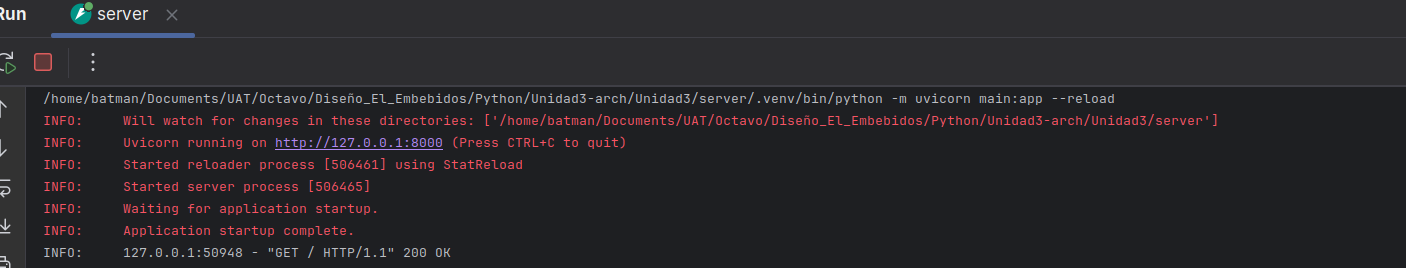
\includegraphics[width=0.8\textwidth]{imagen1}
    \caption{Configuración del entorno de desarrollo}
    \label{fig:configuracion}
\end{figure}

\section{Ejecución del Servidor}

\begin{figure}[h]
    \centering
    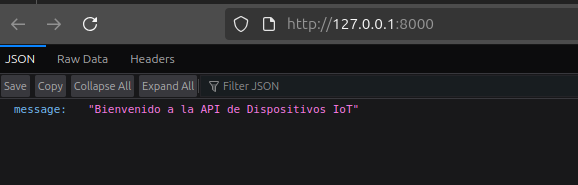
\includegraphics[width=0.8\textwidth]{imagen2}
    \caption{Servidor FastAPI en ejecución}
    \label{fig:servidor}
\end{figure}

\section{Pruebas de Endpoints}

\begin{figure}[h]
    \centering
    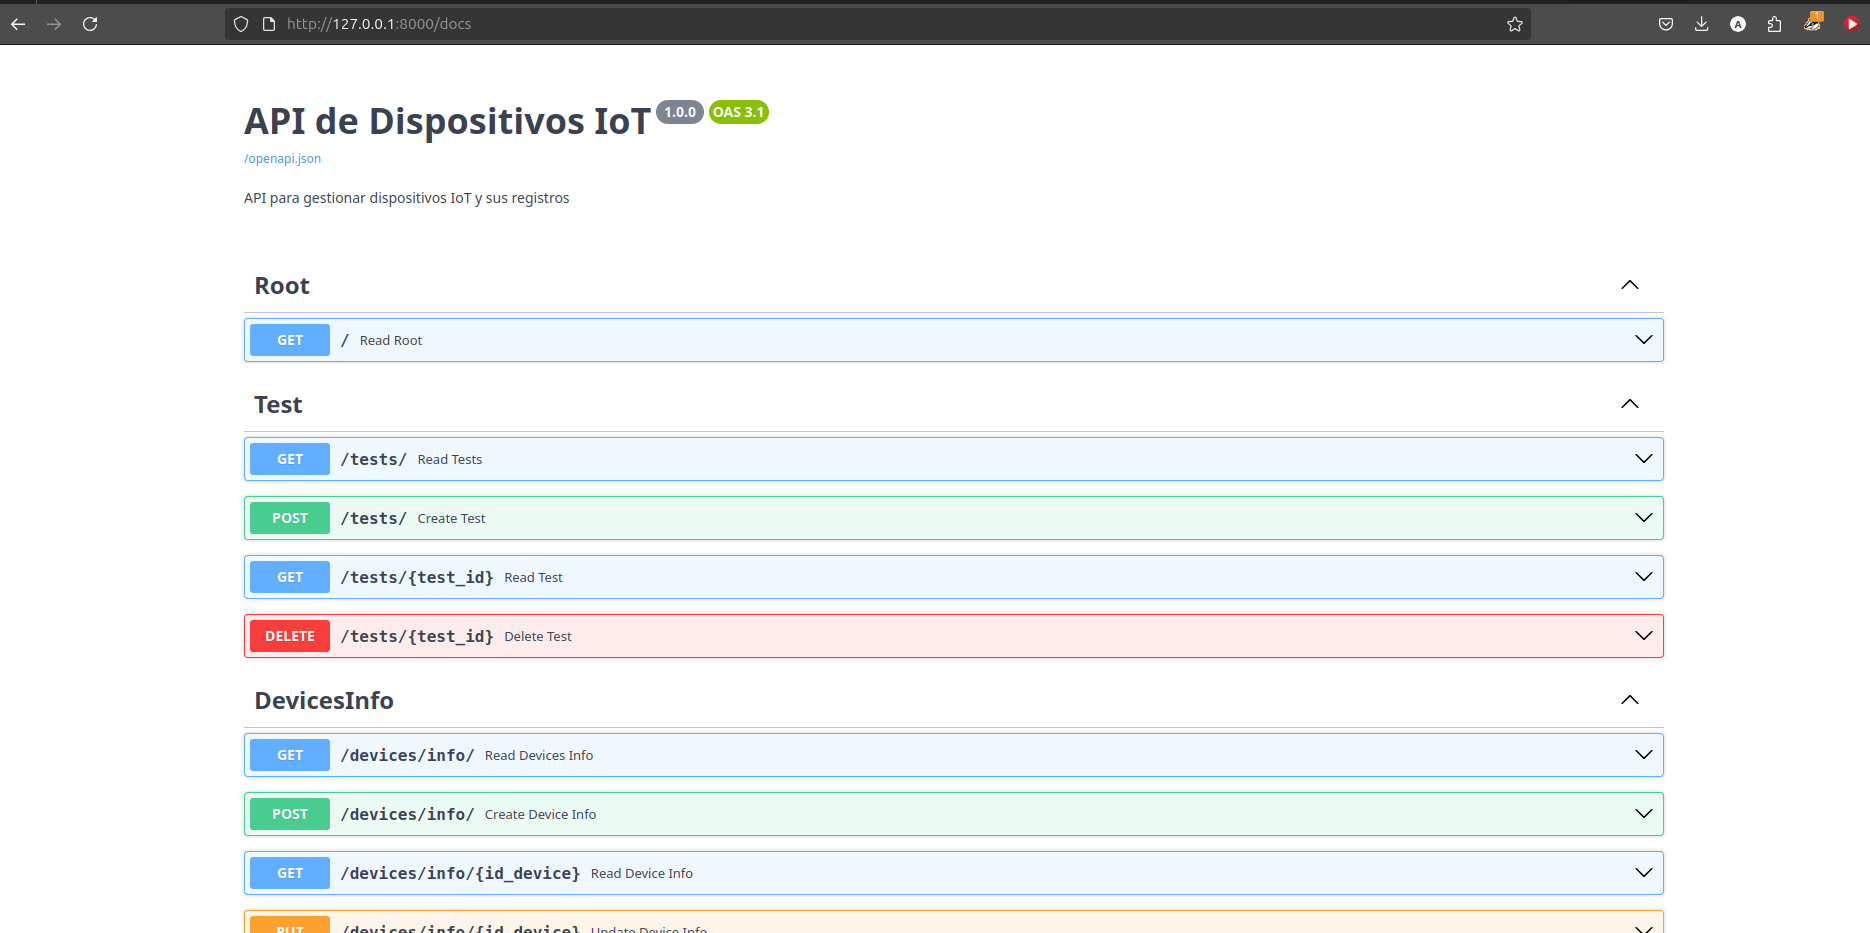
\includegraphics[width=0.8\textwidth]{imagen3}
    \caption{Prueba del endpoint GET /devices/info/}
    \label{fig:endpoint1}
\end{figure}

\begin{figure}[h]
    \centering
    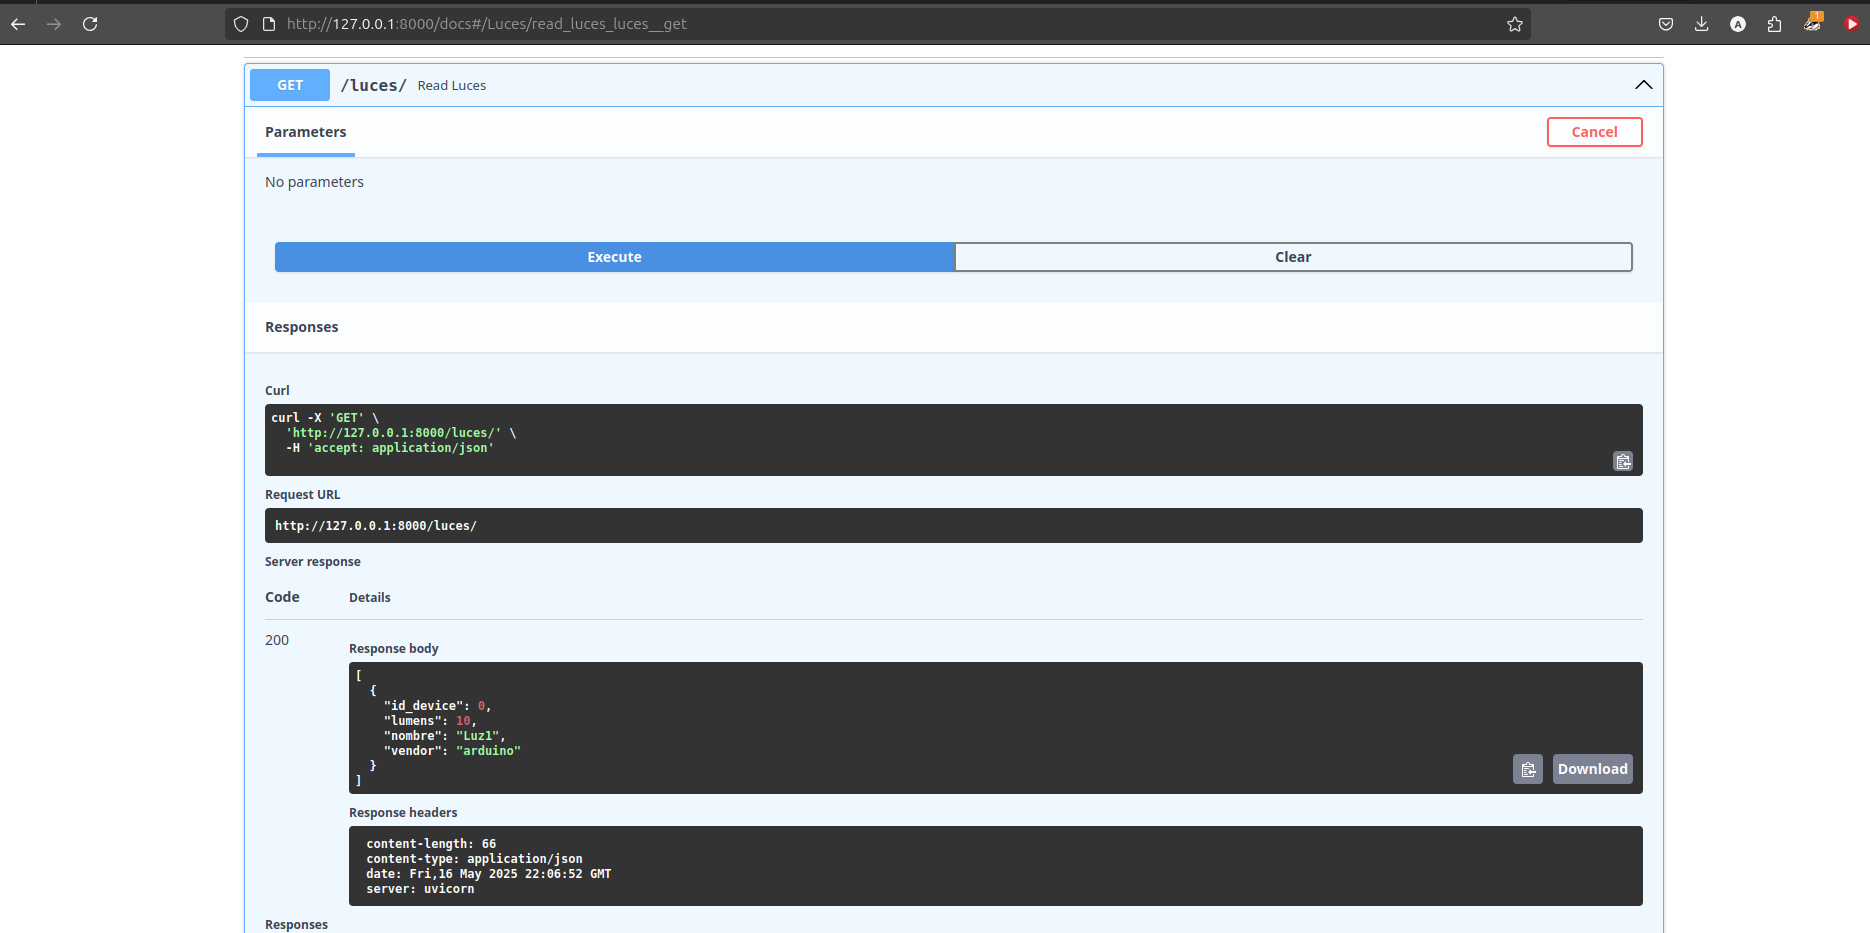
\includegraphics[width=0.8\textwidth]{imagen4}
    \caption{Prueba del endpoint POST /devices/info/}
    \label{fig:endpoint2}
\end{figure}

\section{Documentación Swagger}

\begin{figure}[h]
    \centering
    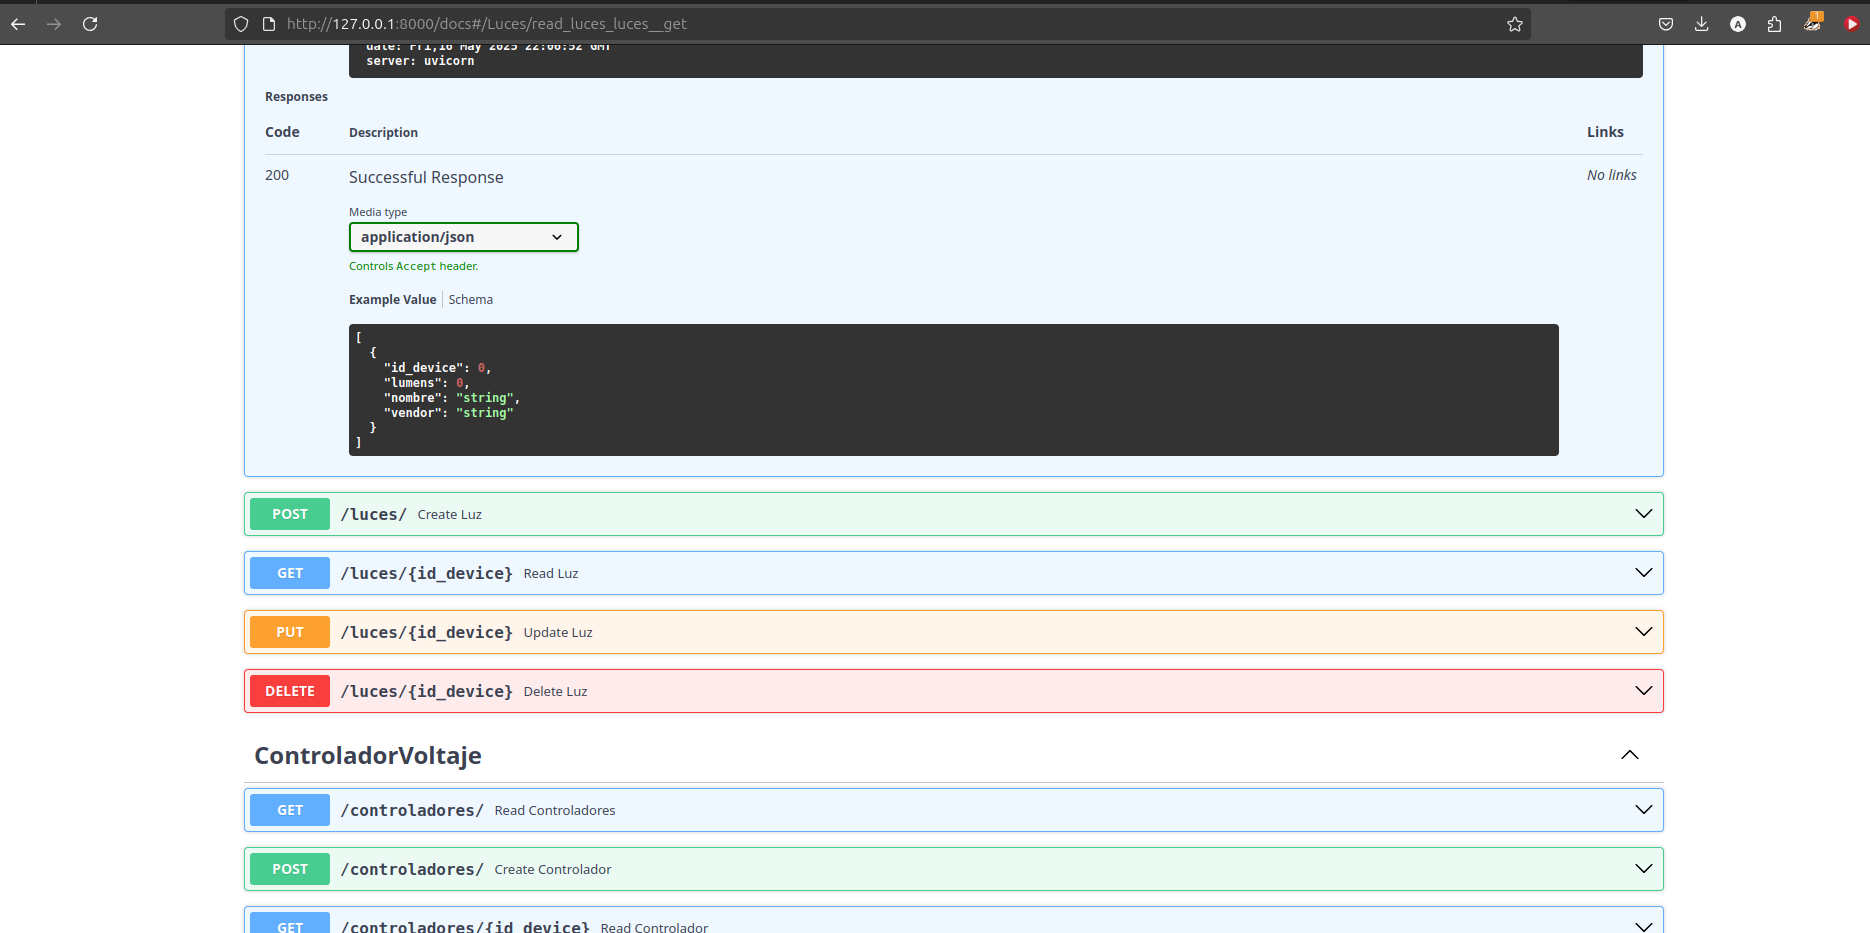
\includegraphics[width=0.8\textwidth]{imagen5}
    \caption{Interfaz de Swagger UI mostrando la documentación interactiva}
    \label{fig:swagger}
\end{figure}

\section{Resultados de Consultas}

\begin{figure}[h]
    \centering
    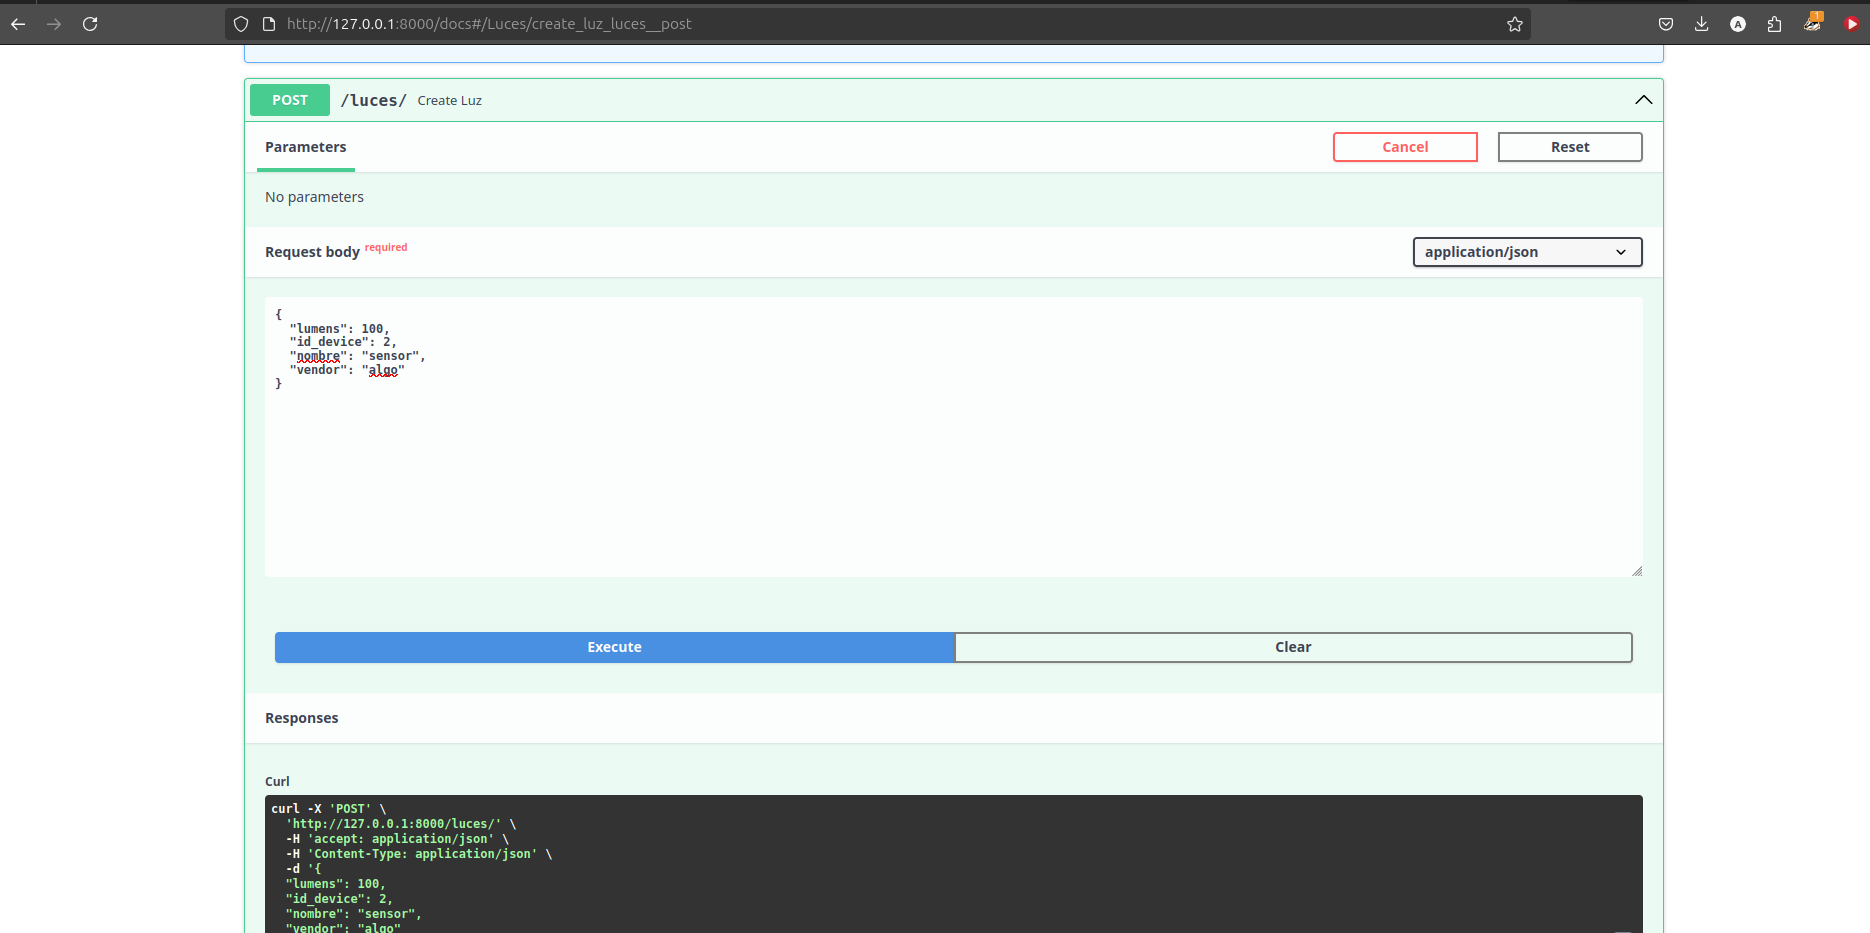
\includegraphics[width=0.8\textwidth]{imagen6}
    \caption{Resultados de consultas a la base de datos}
    \label{fig:resultados}
\end{figure}

% Puedes añadir más secciones según sea necesario para mostrar diferentes aspectos de la ejecución del código

\section{Conclusiones sobre la Evidencia Visual}

Las capturas de pantalla y evidencias visuales presentadas en este capítulo demuestran el funcionamiento correcto de la API de Dispositivos IoT en diferentes escenarios. Estas imágenes no solo validan la implementación descrita en los capítulos anteriores, sino que también sirven como guía visual para los usuarios que deseen replicar la configuración o entender mejor el comportamiento del sistema.

La evidencia visual es particularmente útil para:
\begin{itemize}
    \item Verificar que la API responde correctamente a las solicitudes
    \item Comprobar el formato de las respuestas JSON
    \item Visualizar la interfaz de documentación interactiva
    \item Confirmar el correcto almacenamiento y recuperación de datos
    \item Entender el flujo de trabajo completo del sistema
\end{itemize}

Estas imágenes complementan la documentación técnica y proporcionan una referencia visual que facilita la comprensión del sistema en su conjunto.

\chapter{Documentación Interactiva}

FastAPI genera automáticamente documentación interactiva para la API. Una vez que el servidor está en funcionamiento, puedes acceder a:

\begin{itemize}
    \item \textbf{Swagger UI:} \url{http://localhost:8000/docs}
    \item \textbf{ReDoc:} \url{http://localhost:8000/redoc}
\end{itemize}

Estas interfaces te permiten:

\begin{itemize}
    \item Explorar todos los endpoints disponibles
    \item Ver los esquemas de solicitud y respuesta
    \item Probar los endpoints directamente desde el navegador
    \item Entender los posibles códigos de estado y respuestas de error
\end{itemize}

\chapter{Buenas Prácticas y Recomendaciones}

\section{Manejo de Errores}
La API implementa manejo de errores estándar utilizando códigos de estado HTTP:

\begin{itemize}
    \item \textbf{200 OK:} Solicitud exitosa
    \item \textbf{201 Created:} Recurso creado exitosamente
    \item \textbf{204 No Content:} Solicitud exitosa sin contenido de respuesta (usado para DELETE)
    \item \textbf{404 Not Found:} Recurso no encontrado
    \item \textbf{422 Unprocessable Entity:} Datos de solicitud inválidos
\end{itemize}

\section{Seguridad}
Para mejorar la seguridad de la API, considera implementar:

\begin{itemize}
    \item Autenticación (OAuth2, JWT)
    \item Autorización basada en roles
    \item HTTPS para cifrar las comunicaciones
    \item Limitación de tasa para prevenir ataques de fuerza bruta
    \item Validación de entrada para prevenir inyecciones
\end{itemize}

\section{Escalabilidad}
Para mejorar la escalabilidad de la API, considera:

\begin{itemize}
    \item Implementar caché para respuestas frecuentes
    \item Utilizar bases de datos más robustas para producción (PostgreSQL, MySQL)
    \item Configurar un balanceador de carga para distribuir el tráfico
    \item Implementar un sistema de colas para tareas asíncronas
\end{itemize}

\chapter{Conclusiones}

La API de Dispositivos IoT proporciona una solución completa para la gestión de dispositivos IoT y sus datos. Utilizando FastAPI, se ha creado una API moderna, rápida y fácil de usar que sigue las mejores prácticas de desarrollo.

Las principales ventajas de esta implementación incluyen:

\begin{itemize}
    \item Rendimiento de alta velocidad gracias a FastAPI
    \item Validación automática de datos con Pydantic
    \item Documentación interactiva generada automáticamente
    \item Estructura modular y fácil de mantener
    \item Soporte para diferentes tipos de dispositivos IoT
\end{itemize}

Esta API puede servir como base para sistemas más complejos de IoT, integrándose con otras tecnologías como sistemas de análisis de datos, interfaces de usuario o servicios en la nube.

\end{document}
